\begin{ledgroupsized}[r]{120mm}
\footnotesize 
\pstart 
\noindent\textbf{\"{U}berlieferung:}
\pend
\end{ledgroupsized} 
\begin{ledgroupsized}[r]{114mm}
\footnotesize 
\pstart \parindent -6mm
\makebox[6mm][l]{\textit{L}}Konzept: LH XXXVII 5 Bl. 201, 204. 1 Bog. 2\textsuperscript{o}. 2 S. auf Bl. 201. Bl. 204~r\textsuperscript{o} ist leer. Bl.~204~v\textsuperscript{o} überliefert N. 20. % F/2 = 037,05_204
Der Bog. umschließt zudem Bl. 202-203 (N. 21). % F/3 = 037,05_202-203
Ein Wasserzeichen auf Bl. 201.\\
Cc 2, Nr. 971 A
\pend
\end{ledgroupsized}
%
\vspace{4mm}
\begin{ledgroup}
\footnotesize 
\pstart
\noindent\footnotesize{\textbf{Datierungsgr\"{u}nde}: Leibniz setzt sich im vorliegenden Stück mit Galileis Überlegungen über die Bruch\-festigkeit von Balken aus dem zweiten Dialog der \textit{Discorsi e dimostrazioni matematiche} auseinander, die er in der ersten Ausgabe von Galileis Werken gelesen hat (\cite{01084}G. \textsc{Galilei}, \textit{Opere}, Bd. II, Bologna 1656), wie u.a. ein Verweis im Text belegt (siehe unten, S. \refpassage{37.05_201r_a1}{37.05_201r_a2}). Am Rande von Bl. 201~r\textsuperscript{o} hat Leibniz selbst später vermerkt, er sei noch \glqq ein Anfänger\grqq(\textit{novus}) gewesen, als er das vorliegende Stück verfasst habe. Seine frühe Rezeption der \textit{Discorsi} ist ebenfalls in \cite{00260}\textit{LSB} VI, 3 N. 11\textsubscript{1} und N. 11\textsubscript{2} dokumentiert, wobei N.~11\textsubscript{1} insbesondere auf Galileis Ansichten über die Bruchfestigkeit Bezug nimmt. Dieses Stück, das auf den Herbst 1672 bis zum Winter 1672-1673 datiert worden ist (siehe die Begründung in \textit{LSB} VI, 3, S. 163), ist auf einem Bogen (LH XXXVII 5, Bl. 205-206) überliefert, welcher das gleiche Wasserzeichen aufweist wie Bl. 201. Die Verwandtschaft der Textträger sowie der starke inhaltliche Zusammenhang legen nahe, die Datierung von \cite{00260}\textit{LSB} VI, 3 N. 11 auch für das vorliegende Stück N. 19 % F/1 = 037,05_201
zu übernehmen.}
\pend
\end{ledgroup}
%
\vspace{4mm}
\count\Afootins=1200
\count\Bfootins=1200
\count\Cfootins=1200
\pstart
\noindent
[201~r\textsuperscript{o}]
\pend
\pstart 
\normalsize
\noindent
\centering
\edtext{De}{\lemma{}\Afootnote{\textit{Am oberen Blattrand}: Cum ista scriberem eram in his novus.\vspace{-8mm}}}
\edtext{quibusdam circa Resistentiam,\protect\index{Sachverzeichnis}{resistentia}}{\lemma{De}\Bfootnote{\textit{(1)}\ iis \textit{(2)}\ quibusdam circa Resistentiam \textit{L}}}
quae \edtext{a Galilaeo\protect\index{Namensregister}{\textso{Galilei} (Galilaeus, Galileus), Galileo 1564-1642}}{\lemma{a Galilaeo}\Cfootnote{\cite{00050}G. \textsc{Galilei}, \textit{Discorsi}, Leiden 1638, S. 132ff.
%-146 
(\cite{00048}\textit{GO} VIII, S. 172ff.%
%-186
).}}
aut non aut sine demonstratione,\\
aut secus \edtext{quam res postulet}{\lemma{quam res postulet}\Bfootnote{\textit{erg. L}}}, dicuntur.
\pend
\vspace{0.8em}
\pstart
\noindent
Non demonstrat rupturam\protect\index{Sachverzeichnis}{ruptura} incipere in uno
\edtext{puncto; neque}{\lemma{puncto;}\Bfootnote{\textit{(1)}\ non \textit{(2)}\ neque\textit{ L}}}
dicit neque demonstrat distantias punctorum sectionis
\edtext{rupturae\protect\index{Sachverzeichnis}{ruptura} esse}{\lemma{rupturae}\Bfootnote{\textit{(1)}\ ad \textit{(2)}\ esse \textit{L}}}
in ratione \edtext{resistentiae\protect\index{Sachverzeichnis}{resistentia}}{\lemma{resistentiae}\Bfootnote{\textit{erg. L}}}
distantiarum a puncto
\pend
\newpage
\pstart \noindent divulsionis:\protect\index{Sachverzeichnis}{divulsio}
nec \edtext{tetigit rectas}{\lemma{tetigit}\Bfootnote{\textit{(1)}\ lineas \textit{(a)}\ resistent \textit{(b)}\ sectionum \textit{(2)}\ rectas \textit{L}}}
a centro divulsionis\protect\index{Sachverzeichnis}{centrum divulsionis} eductas esse[,] quod ad resistentias[,] inter se, ut quadrata.
Unde sequitur, triangulum habere resistentiam\protect\index{Sachverzeichnis}{resistentia} parabolae.\protect\index{Sachverzeichnis}{parabola}
%\edtext{}{\lemma{Unde [...] parabolae}\Cfootnote{\cite{00050}a.a.O., S. ??? (\cite{00048}\textit{GO} VIII, S. ???.).}}
Nec methodum\protect\index{Sachverzeichnis}{methodus} attigit generalem, dato uno experimento\protect\index{Sachverzeichnis}{experimentum} caetera omnia \edtext{in eadem materia}{\lemma{omnia}\Bfootnote{\textit{(1)}\ in calculandi perf \textit{(2)}\ in eadem materia \textit{L}}} determinandi sine calculo, per simplicem stateram.\protect\index{Sachverzeichnis}{statera}
\pend
\pstart
Quae vero
\edtext{de ruptura\protect\index{Sachverzeichnis}{ruptura}
\edtext{baculi\protect\index{Sachverzeichnis}{baculus}}{\lemma{ruptura}\Bfootnote{\textit{(1)}\ trabis \textit{(2)}\ baculi \textit{L}}}
super genu vel trabis\protect\index{Sachverzeichnis}{trabs} super fulcro\protect\index{Sachverzeichnis}{fulcrum} dicit,}{\lemma{de ruptura [...] dicit}\Cfootnote{\cite{00050}a.a.O., S. 133f. (\cite{00048}\textit{GO} VIII, S. 173f.).}}
iis ne assentiri quidem possum.
\pend
\pstart
\edtext{Putat enim si datis quibusdam viribus\protect\index{Sachverzeichnis}{vis} opus sit ad frangendum,
fulcro in medio posito,
fieri posse ut nec centuplum sufficiat,
fulcro\protect\index{Sachverzeichnis}{fulcrum} in alio quodam puncto posito,
imo ut infinituplo opus sit, quod probare conatur
\edlabel{37.05_201r_b1}\edtext{}{{\xxref{37.05_201r_b1}{37.05_201r_b2}}\lemma{}\Bfootnote{prop.\ \textbar\ p. \textit{erg. Hrsg.}\ \textbar\ 102. \textit{(1)}\ argumento paralogistico \textit{(2)}\ paralogismo \textit{L}}}\edlabel{37.05_201r_a1}\edtext{prop. [p.] 102.}{\lemma{prop. [p.] 102}\Cfootnote{Die Angabe bezieht sich auf \cite{01084}G. \textsc{Galilei}, \textit{Discorsi}, Bologna 1656 (\textit{Opere}, Bd. II), S. 102 (\cite{00048}\textit{GO} VIII, S. 176).
Dass Leibniz zu Beginn seines Pariser Aufenthaltes diese Ausgabe der \textit{Discorsi} gelesen hat, entnimmt man \textit{LSB} VI, 3 N. 11\textsubscript{1}, S. 163f. und N. 11\textsubscript{2}, S. 167f.\cite{00260}}}}{\lemma{Putat [...] 102}\Cfootnote{\cite{00050}a.a.O., S. 134-136 (\cite{00048}\textit{GO} VIII, S. 174-176).}}
paralogismo\edlabel{37.05_201r_a2}\edlabel{37.05_201r_b2}
quem miror excidere potuisse tanto viro.\label{037,05_201}
\pend
\pstart
Ponatur resistentia trabis\protect\index{Sachverzeichnis}{resistentia trabis} fultae in $C$ seu pondera\protect\index{Sachverzeichnis}{pondus} ad eam rumpendam sufficientia $A+B.$ esse quantacunque fulcro $C$ moto versus $A$ ut \edtext{in $CC$}{\lemma{in}\Bfootnote{\textit{(1)}\ $F$ \textit{(2)}\ $CC$ \textit{L}}}[,]
minuetur \edtext{potentia\protect\index{Sachverzeichnis}{potentia} $A$ continue}{\lemma{}\Bfootnote{potentia $A$\ \textbar\ vel $E$ \textit{gestr.}\ \textbar\ continue \textit{L}}} et quidem in infinitum.\protect\index{Sachverzeichnis}{infinitum}
Necesse \edtext{ergo est}{\lemma{ergo}\Bfootnote{\textit{(1)}\ esset \textit{(2)}\ est \textit{L}}} potentiam $B$ augeri \edtext{[in]}{\lemma{in}\Bfootnote{\textit{erg. Hrsg.}}} infinitum,
ut diminuta altera $A$ in infinitum, nihilominus summa resistentiae trabis aequivaleat, at non augetur in infinitum potentia $BB$ remoto licet fulcro $C$ \edtext{tota}{\lemma{$C$}\Bfootnote{\textit{(1)}\ usque \textit{(2)}\ tota \textit{L}}} trabis longitudine. Ergo potentia\protect\index{Sachverzeichnis}{potentia} $A+B$ altera in infinitum minuta, sed altera non in infinitum aucta, non ut ante resistentiae Trabis aequivalebunt, sed resistentia trabis\protect\index{Sachverzeichnis}{resistentia trabis} erit aucta. Ecce argumentum, quo audito\hfill
\edtext{collocutor}{\lemma{\hspace{1.8mm}18-S.167.2\hspace{1.8mm}collocutor [...] infinito}\killnumber\Cfootnote{\cite{00050}G. \textsc{Galilei}, \textit{Discorsi}, Leiden 1638, S. 135 (\cite{00048}\textit{GO} VIII, S. 175).}}\hfill exclamat,\hfill
\edtext{[se]}{\lemma{sed}\Bfootnote{\textit{L ändert Hrsg.}}}\hfill
\setline{16}admirari\hfill vim\hfill Geometriae\hfill tam\hfill inexpectata\hfill eruentis,\hfill
se
\pend
\vspace{1.5em}
%%%%%%%
\pstart
\centering
\noindent
%\begin{wrapfigure}[8]{l}{0.55\textwidth}
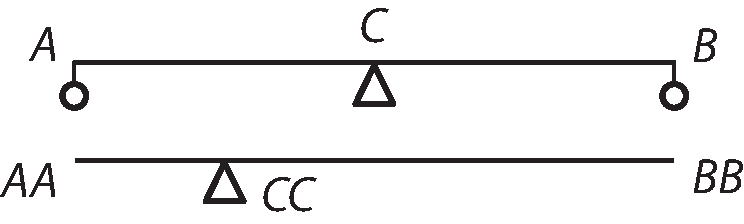
\includegraphics[trim = 0mm -2mm 0mm 0mm, clip,width=0.44\textwidth]{images/lh03705_201r-d1.pdf}\\
\centering
%\vspace*{0.2em}
%\newline
%\rule[0mm]{30mm}{10mm}
[\textit{Fig. 1}]
\pend
\count\Afootins=1200
\count\Bfootins=1200
\count\Cfootins=1200
\newpage
\pstart
\noindent
enim crediturum
\edtext{fuisse, resistentiam}{\lemma{fuisse,}\Bfootnote{\textit{(1)}\ potentiam \textit{(2)}\ resistentiam \textit{L}}}
manere eandem, at fuisse deceptum, non parum, sed integro infinito.
\edtext{Sed ego}{\lemma{Sed}\Bfootnote{\textit{(1)}\ ut \textit{(2)}\ mihi \textit{(3)}\ ego \textit{L}}}
repetere cogor, nescire me quomodo talia exciderint tanto viro.
Primum enim si potentia $B$ in infinitum augenda est, potentia $A$ in infinitum minuta seu fulcro $C$ ipsi supposito, quo casu \edtext{potentia $A$}{\lemma{potentia}\Bfootnote{\textit{(1)}\ $B$ \textit{(2)}\ $A$ \textit{L}}} evanescit, sequetur fulcro\protect\index{Sachverzeichnis}{fulcrum} posito in $A$ potentia $A$ remota, potentiam\ $B$ ad trabem\protect\index{Sachverzeichnis}{trabs} in $A$ rumpendam esse
\edtext{debere infinitam,}{%
\lemma{}%
\Bfootnote{debere\ \textbar\ in \textit{streicht Hrsg.}\ \textbar\ infinitam,}}
quod est absurdum. Sed et facile retextu sophisma
\edtext{est: Cum}{\lemma{est:}\Bfootnote{\textit{(1)}\ Dicit \textit{(2)}\ Fateor \textit{(3)}\ Cum \textit{L}}}
duae sint potentiae 
\edtext{$A+B,$ concedo}{\lemma{$A+B,$}\Bfootnote{\textit{(1)}\ fateor, ut quantum minuitur \textit{(2)}\ concedo \textit{L}}}
Galilaeo,\protect\index{Namensregister}{\textso{Galilei} (Galilaeus, Galileus), Galileo 1564-1642}
si \edtext{mutato fulcro}{\lemma{mutato fulcro}\Bfootnote{\textit{erg. L}}}
una in \edtext{infinitum minuatur,}{\lemma{infinitum}\Bfootnote{\textit{(1)}\ augeatur \textit{(2)}\ minuatur \textit{L}}}
alteram in infinitum
\edtext{esse augendam.}{\lemma{esse}\Bfootnote{\textit{(1)}\ minuendam \textit{(2)}\ augendam \textit{L}}}%
\protect\index{Sachverzeichnis}{infinitum}\protect\index{Sachverzeichnis}{fulcrum}\protect\index{Sachverzeichnis}{potentia}
Sed cur?
Nonne, ut summa
\edtext{potentiarum}{\lemma{potentiarum}\Bfootnote{\textit{erg. L}}}
maneat eadem,
quia scilicet resistentia manet eadem.
En ergo \edtext{resistentiam\protect\index{Sachverzeichnis}{resistentia trabis}
trabis}{\lemma{resistentiam}\Bfootnote{\textit{(1)}\ fulcrorum \textit{(2)}\ trabis \textit{L}}}
fulcro utcunque mutato eandem manere[,]
suppositum ab ipso
Galilaeo\protect\index{Namensregister}{\textso{Galilei} (Galilaeus, Galileus), Galileo 1564-1642}
velut fundamentum demonstrationis,
qua contrarium probare nititur.
Jam probationem consideremus:
Si mutato \edtext{fulcro potentia $A$ in infinitum}{\lemma{fulcro}\Bfootnote{\textit{(1)}\ in in \textit{(2)}\ potentia $A$ in infinitum \textit{L}}}
minuatur, potentia $B$ in infinitum augenda est.
At verum est prius. \edtext{Probat:
\edtext{nam fulcro $C$ ad dimidiam}{\lemma{nam}\Bfootnote{\textit{(1)}\ cum \textit{(2)}\ fulcro \textbar\ $C$ \textit{erg.} \textbar\ ad dimidiam \textit{L}}}
 $AC$ perveniente $A$ dimidiatur,
ad \edtext{quartam, assumitur}{\lemma{quartam,}\Bfootnote{\textit{(1)}\ $A$ dim \textit{(2)}\ assumitur \textit{L}}}
quinta de $A$ et sic in infinitum,
ut fulcro perveniente
\edtext{in $A$ potentia}{\lemma{in $A$}\Bfootnote{\textit{(1)}\ summa hi \textit{(2)}\ potentia \textit{L}}}
fiat pars infinitesima\protect\index{Sachverzeichnis}{pars infinitesima} de $A$ seu evanescat.\protect\index{Sachverzeichnis}{pars infinitesima}
Ergo $B$ in infinitum augenda est, seu fiet infinita.}{\lemma{Probat: [...] infinita}\Cfootnote{\cite{00050}a.a.O., S. 134f. (\cite{00048}\textit{GO} VIII, S. 174f.).
Zu Beginn von N. 21 % F/3 = 037,05_202-203
wird diese Stelle zum Teil ins Lateinische übersetzt und Satz für Satz kommentiert.}}
Respondetur minui aliquid in infinitum dupliciter intelligi potest, vel ipsum dividi et subdividi in infinitum, vel aliquod infinitum ei subtrahi. Hoc loco nullum infinitum \edtext{subtrahitur a potentia}{\lemma{subtrahitur}\Bfootnote{\textit{(1)}\ ab \textit{(2)}\ a potentia \textit{L}}} $A$ sed potentia $A$ subdividitur tantum in infinitum.\protect\index{Sachverzeichnis}{infinitum}\protect\index{Sachverzeichnis}{potetntia}\protect\index{Sachverzeichnis}{resistentia}
Jam si duae sint quantitates, et una in infinitum dividatur, non est necesse alteram in infinitum multiplicari, ut summa maneat eadem, imo contra hoc modo summa non manebit \edtext{eadem. Esto}{\lemma{eadem.}\Bfootnote{\textit{(1)}\ Sunt \textit{(2)}\ Sunto \textit{(3)}\ Esto \textit{L}}} enim \edtext{$a+b$. Patet}{\lemma{$a+b$.}\Bfootnote{\textit{(1)}\ Ergo \textit{(2)}\ Patet \textit{L}}} \rule[-4mm]{0mm}{10mm}${\displaystyle\frac{a}{2} + 2b}$ non esse ei aequale. \rule[-4mm]{0mm}{10mm}${\displaystyle a+b = \frac{a}{2} + 2b}$. Ergo $2a+2b=a+4b$. Ergo $2a=a+2b$. Ergo $a=2b$. Ergo si duae sint quan-%
\pend
\newpage
\pstart
\noindent%
titates, et una dimidiata, alteraque duplicata, summa aequivalet summae priori, necesse est dimidiam duplicatae fuisse
\edtext{duplam.
[201~v\textsuperscript{o}]
% \newline\hspace*{7,5mm}
Et ecce}{%
\lemma{duplam.}\Bfootnote{%
\textit{(1)} Et in genere, quoties hoc contingit ea debet ratio imminutionis unius et augmenti alterius, quae est ratio imminuendae. Et ecce ad augendam per hanc demonstrationem generalem: $\displaystyle a+b = \frac{a}{1r} + 1rb$. Ergo $1ra+1rb= a+1rqb$. Ergo $1ra-a=1rqb-b$ seu differentia inter augendum et auctum debet esse aequalis differentiae minuendi in se ipsum seu quadratum rationis multiplicati [201~v\textsuperscript{o}]
\textit{(a)}\ seu
\textit{(aa)}\ si
\textit{(bb)}\ generaliter si post multiplicationem unius, et
\textit{(aaa)}\
ad \textit{(bbb)}\
divisionem alterius servatur nihilominus aequalitas summarum
\textit{(2)}\ $1ra-a=1rqb-b$. seu $1r-1,\smallfrown a=1rq-1,\smallfrown b$. Ergo $\displaystyle 1r-1=1rq-1,\smallfrown \frac{b}{a}$. Ergo: $\displaystyle\frac{1r-1}{1rq-1.}=\frac{b}{a}$. \textit{(3)} Et ecce \textit{L}}}
per demonstrationem generalem:
\pend
%
\vspace*{0.5em}% PR: Rein provisorisch !!!
\pstart%
\noindent%
%
%
%
\hspace*{96,25mm}%
16%
\newline%
\setline{1}\hspace*{91,5mm}%
$\displaystyle 8 \overgroup{\phantom{aaiiicc}}$%
\newline%
$\displaystyle 8 \overgroup{\phantom{ac}} 4$%
\hspace*{10,0mm}%
$\displaystyle 4 \overgroup{\phantom{ac}} 8$%
\hspace*{19,5mm}%
$\displaystyle 16 \overgroup{\phantom{ac}} 8$%
\hspace*{7,5mm}%
$\displaystyle 8 \overgroup{\phantom{ac}} 16$%
\hspace*{18,5mm}%
$\displaystyle 16 \overgroup{\phantom{ac}} 8$%
\hspace*{7,0mm}%
8\hspace*{4,0mm}16%
\newline%
$\displaystyle a + b = \displaystyle\frac{a}{(2)1r}+b1r.$
%
%
\quad Ergo
%
$\displaystyle 1ra + 1rb = a + 1rqb.$
%
%
\quad Ergo
%
$\displaystyle 1ra - a + 1rb = 1rqb.$
%
\pend
%
%
\vspace*{1.0em}% PR: Rein provisorisch !!!
\pstart%
\noindent%
\hspace*{14,25mm}%
8%
\hspace*{70,25mm}%
8%
\newline%
\hspace*{10,0mm}%
\setline{1}$\displaystyle 16 \overgroup{\phantom{ac}} 8$%
\hspace*{7,0mm}%
16%
\hspace*{3,5mm}%
8%
\hspace*{21,5mm}%
8%
\hspace*{19,75mm}%
$\displaystyle 16 \overgroup{\phantom{aaaiiccc}} 8$%
\newline%
Ergo
$\displaystyle 1ra - a = 1rqb - 1rb.$
%
%
\setline{4}\quad Ergo
%
\edtext{$\displaystyle 1r - 1, \smallfrown a = 1r \smallfrown 1r \smallfrown b - 1r \smallfrown b.$%
}{\lemma{$\displaystyle 1r - 1, \smallfrown a =$}\Bfootnote{\textit{(1)}\ $\displaystyle 1rq$  \textit{(2)}\ $\displaystyle 1rb \smallfrown 1rb$  \textit{(3)}\ $\displaystyle 1r \smallfrown 1r \smallfrown b1r \smallfrown b.$ \textit{L}}}
\pend
%
\vspace*{1.0em}% PR: Rein provisorisch !!!
\pstart%
\noindent%
\setline{4}\hspace*{15,5mm}%
8%
\hspace*{12,0mm}%
$\displaystyle 8 \overgroup{\phantom{aaiicc}} 1$%
\hspace*{22,0mm}%
1%
\hspace*{37,0mm}%
$\frac{1}{2} \overgroup{\phantom{\frac{i}{i}}} \scriptstyle 2 \textstyle \left( \frac{2}{2} = \scriptstyle 1 \right) \scriptstyle 1$
\newline%
Ergo
%
\edtext{$\displaystyle 1r - 1, \smallfrown a = 1rb \smallfrown \llcorner 1r - 1.$%
}{\lemma{$\displaystyle 1r - 1, \smallfrown a =$}\Bfootnote{\textit{(1)} $\displaystyle 1r \smallfrown br \smallfrown 1r - 1, +$ \textit{(2)} $\displaystyle 1rb \smallfrown \llcorner 1r - 1.$ \textit{ L}}} 
%
\quad Ergo
%
$\displaystyle 1r - 1 = \left(\frac{b}{a} \smallfrown \llcorner \llcorner 1r \smallfrown 1r - 1\right) \frac{b}{a} \smallfrown 1rq - 1r.$
%
\pend
\vspace*{1.0em}% PR: Rein provisorisch !!!
\pstart%
\noindent%
Ergo
% \rule[-5mm]{0pt}{12mm}
${\displaystyle \left(\frac{1}{2}\right) \frac{1r - 1}{1rq - 1r} = \frac{b}{a}}$%
\edtext{}{\lemma{}\Afootnote{\textit{Am Rand}: $a$ minuenda, $b$ augenda[,] $1r$ ratio augmenti vel diminutionis.\vspace{-4mm}}}.
\pend
\vspace{1.0em}% PR: Rein provisorisch !!!
% \newpage% PR: Rein provisorisch !!!
\pstart
Regula ergo haec est, \edtext{si duabus quantitatibus altera aucta}{\lemma{si}\Bfootnote{%
\textit{(1)}\ non duab %
\textit{(2)}\ duabus quantitatibus altera %
\textit{(a)}\ non %
\textit{(b)}\ aucta \textit{L}}} altera minuta, in ratione eadem; summa productorum aequalis est summae quantitatum; necesse est rationem augendae ad minuendam esse, ut ratio augmenti \edtext{diminutionisve minuta unitate}{\lemma{diminutionisve}\Bfootnote{\textit{(1)}\ aucta unit \textit{(2)}\ minuta unitate \textit{L}}} ad quadratum suum etiam minutum unitate.
\pend
\newpage
\pstart
Eodem \edtext{modo inveniemus}{\lemma{modo}\Bfootnote{\textit{(1)}\ calculabitur \textit{(2)}\ inveniemus \textit{L}}} regulam, ut differentiae quantitatum sint aequales differentiae productorum, item, ut summae vel differentiae non quidem sint aequales habeant tamen rationem datam.
\pend
\pstart
Ex his apparet, minime necesse esse, ad id ut summa \edtext{productorum}{\lemma{}\Bfootnote{productorum \textit{erg.} \textit{L}}} maneat eadem duas quantitates in eadem ratione ut unam augeri, ita alteram minui neque enim id contingere, nisi quando ea est ratio quantitatum, quae rationis unitate multatae ad quadratum suum unitate minutum. \edtext{Ac}{\lemma{minutum.}\Bfootnote{\textit{(1)}\ Quare non est \textit{(2)}\ Ac \textit{L}}} proinde duas quantitates propositas \edtext{hoc}{\lemma{propositas}\Bfootnote{\textit{(1)}\ id \textit{(2)}\ hoc \textit{L}}} praestituras, tantum in ratione augmenti diminutionisve certa, nullas capaces esse, ut hoc praestent in ratione assumta \edlabel{quibusdam1}quacunqe.
\pend
\pstart
\edtext{Caeterum\edlabel{quibusdam2}}{{\xxref{quibusdam1}{quibusdam2}}\lemma{quacunque.}\Bfootnote{\textit{(1)}\ Quam ex \textit{(2)}\ Caeterum \textit{L}}}
Galilaeus\protect\index{Namensregister}{\textso{Galilei} (Galilaeus, Galileus), Galileo 1564-1642}
his suis quasi serio demonstratis nixus,
etiam \edtext{conatur rationem mutatarum pro mutato fulcri loco differentiarum assignare,}{\lemma{conatur [...] assignare}\Cfootnote{\cite{00050}a.a.O., S. 135f. (\cite{00048}\textit{GO} VIII, S. 176).}}
sed demonstratione tam obscura,
ut nullo modo sensum intellectus capacem eruere potuerim,
praeterquam quod necesse est propositionem esse
\edtext{falsam. Porro}{\lemma{falsam.}\Bfootnote{\textit{(1)}\ Hinc corruit et problema \textit{(2)}\ Porro \textit{L}}}
cum hactenus ratiocinatus sit de
\edtext{trabe\protect\index{Sachverzeichnis}{trabs} in medio alibive uno in loco fulta, et ponderibus\protect\index{Sachverzeichnis}{pondus} utrinque appensis rumpenda, de improviso }{\lemma{trabe}\Bfootnote{\textit{(1)}\ rumpenda \textit{(2)}\ in medio [...] rumpenda \textit{(a)}\ subito for \textit{(b)}\ transit \textit{(c)}\ de improviso transit \textit{L}}}\edtext{transit ad casum trabis in extremis fultae,
ponderisque nunc in medio nunc alibi
appensi}{\lemma{transit [...] appensi}\Cfootnote{\cite{00050}a.a.O., S.~136 (\cite{00048}\textit{GO} VIII, S. 176). Siehe hierzu N. 20. % F/2 = 037,05_204
}}\edtext{.
Sed consequentiam non [probat].
Hoc enim accurate}{%
\lemma{appensi.}\Bfootnote{%
\textit{(1)}\ Et vero recte, etsi consequentiam non probet.
\textit{(2)}\ Sed consequentiam non\ \textbar\ probet \textit{ändert Hrsg.}\ \textbar .
\textit{(a)}\ Cum enim pondus aequiponderet resistentiis,
idem est duobus ponderibus quaerere,
resistentia in medio assumta,
aut de duabus resistentiis pondere existente utrinque.
Sed hoc accuratius 
\textit{(b)}\ Hoc enim accurate\textit{ L}}}
demonstrandum erat.
Cum tamen id falsum esse videatur,
nam trabe\protect\index{Sachverzeichnis}{trabs} frangenda ex centro,
\edtext{in loco}{\lemma{in}\Bfootnote{\textit{(1)}\ puncto \textit{(2)}\ loco \textit{L}}} appensionis,
\edtext{praeter duas resistentias}{\lemma{praeter}\Bfootnote{\textit{(1)}\ resistentiam \textit{(2)}\ duas resistentias \textit{L}}}
in extremis calculanda est resistentia in medio,\protect\index{Sachverzeichnis}{resistentia centralis} quae crescit cum \edtext{vecte\protect\index{Sachverzeichnis}{vectis} potentiae}{\lemma{vecte}\Bfootnote{\textit{(1)}\ ponderis \textit{(2)}\ potentiae \textit{L}}}, est \edtext{enim celeritas\protect\index{Sachverzeichnis}{celeritas}}{\lemma{enim}\Bfootnote{\textit{(1)}\ ea \textit{(2)}\ celeritas \textit{L}}} motus utriusque potentiae, ex divulsionis\protect\index{Sachverzeichnis}{divulsio} in loco suspensionis eadem. Hinc omne cylindricum habet hoc ut sit ubique aequaliter resistens, si utrinque fultum intelligatur. Imo demonstrabo: in Trabibus utrinque fultis nullum esse calculum ineundum resistentiarum in extremis.
Nam si pondus\protect\index{Sachverzeichnis}{pondus} praevalet simplici cohaesioni\protect\index{Sachverzeichnis}{cohaesio} in ea recta perrumpet, \edtext{sin non praevalet, multo minus}{\lemma{sin}\Bfootnote{\textit{(1)}\ minus \textit{(2)}\ non praevalet, multo minus \textit{L}}} praevalebit majori resistentiae\protect\index{Sachverzeichnis}{resistentia} ex fulcro, nunquam ergo trabs\protect\index{Sachverzeichnis}{trabs} utrinque fulta rumpetur in extremis nunquam motu ex centro, semper \edtext{libero.}{\lemma{libero}\Bfootnote{\textit{(1)}\ , at secus est si ubi utrinque affixa est, affixionis vel \textit{(2)}\ imo contra, si praeponderati \textit{(3)}\ nisi a \textit{(4)}\ . \textit{L}}}
\pend
\count\Afootins=1500
\count\Bfootins=1500
\count\Cfootins=1500
